\documentclass[../main.tex]{subfiles}
\begin{document}
In this chapter, we will specifically talk math related problems. Normally, for the problems appearing in this section, they can be solved using our learned programming methodology. However, it might not inefficient (we will get LTE error on the LeetCode) due to the fact that we are ignoring their math properties which might help us boost the efficiency. Thus, learning some of the most related math knowledge can make our life easier. 
%%%%%%%%%%%%%%%%%%%%%%%%%%%%%%%%%%%%%%%%%%%%%%%%%%%%%%%%%%%%%%%%%%%%%%%%%%%%%%%%
% sorting
%%%%%%%%%%%%%%%%%%%%%%%%%%%%%%%%%%%%%%%%%%%%%%%%%%%%%%%%%%%%%%%%%%%%%%%%%%%%%%%%%%%

%%%%%%%%%%%%%%%%%%%%%%%%%%%%%%%%%%%%%%%%%%%%%%%%%%%%%%%%%%%%%%%%%%%%%%%%%%%%%%%%
% GCD
%%%%%%%%%%%%%%%%%%%%%%%%%%%%%%%%%%%%%%%%%%%%%%%%%%%%%%%%%%%%%%%%%%%%%%%%%%%%%%%%%%%

\section{Numbers}
\subsection{Prime Numbers}
A prime number is an integer greater than 1, which is only divisible by 1 and itself. First few prime numbers are : 2 3 5 7 11 13 17 19 23 ...

Some interesting facts about Prime numbers: 
\begin{enumerate}
    \item 2 is the only even Prime number.
    \item  2, 3 are only two consecutive natural numbers which are prime too.
    \item \label{divide}Every prime number except 2 and 3 can represented in form of 6n+1 or 6n-1, where n is natural number.
    \item \label{godld} Goldbach Conjecture: Every even integer greater than 2 can be expressed as the sum of two primes. Every positive integer can be decomposed into a product of primes.
    \item GCD of a natural number with Prime is always one.
    \item Fermat’s Little Theorem: If n is a prime number, then for every a, $1 <= a < n $, %$a^{(n-1)} == 1 (mod n) OR a^(n-1) % n = 1$. check if it is useful in real situation
    \item Prime Number Theorem : The probability that a given, randomly chosen number n is prime is inversely proportional to its number of digits, or to the logarithm of n.
\end{enumerate}
\subsubsection{Check Single Prime Number}
Learning to check if a number is a prime number is necessary: the naive solution comes from the direct definition, for a number $n$, we try to check if it can be divided by number in range $[2, n-1]$, if it divides, then its not a prime number. 
\begin{lstlisting}[language=Python]
def isPrime(n):
    # Corner case
    if (n <= 1):
        return False
    # Check from 2 to n-1
    for i in range(2, n):
        if (n % i == 0):
            return False
return True
\end{lstlisting}
There are actually a lot of space for us to optimize the algorithm. First, instead of checking till n, we can check till $\sqrt{n}$ because a larger factor of n must be a multiple of smaller factor that has been already checked. Also, because even numbers bigger than 2 are not prime, so the step we can set it to 2. The algorithm can be improved further by use feature \ref{divide} that all primes are of the form $6k \pm 1$, with the exception of 2 and 3.  Together with feature \ref{godld} which implicitly states that every non-prime integer is divisible by a prime number smaller than itself. So a more efficient method is to test if n is divisible by 2 or 3, then to check through all the numbers of form $6k \pm 1$.
\begin{lstlisting}[language=Python]
def isPrime(n):
    # corner cases
    if n <= 1:
        return False
    if n<= 3:
        return True
    
    if n % 2 == 0 or n % 3 == 0:
        return False
        
    for i in range(5, int(n**0.5)+1, 6):  # 6k+1 or 6k-1, step 6, up till sqrt(n), when i=5, check 5 and 7, (k-1, k+1)
        if n%i == 0 or n%(i+2)==0:
            return False
    return True
return True
\end{lstlisting}

\subsubsection{Generate A Range of Prime Numbers}
\paragraph{Wilson theorem} says if a number k is prime then $((k-1)! + 1) \% k$ must be 0. Below is Python implementation of the approach. Note that the solution works in Python because Python supports large integers by default therefore factorial of large numbers can be computed.
\begin{lstlisting}[language=Python]
# Wilson Theorem
def primesInRange(n):
    fact = 1 
    rst = []
    for k in range(2, n):
        fact *= (k-1)
        if (fact + 1)% k == 0:
            rst.append(k)
    return rst
    
print(primesInRange(15)) 
# output
# [2, 3, 5, 7, 11, 13]
\end{lstlisting}

\paragraph{Sieve Of Eratosthenes} To  generate a list of primes. It works by recognizing \textit{Goldbach Conjecture} that all non-prime numbers are divisible by a prime number. An optimization is to only use odd number in the primes list, so that we can save half space and half time. The only difference is we need to do index mapping.
\begin{lstlisting}[language=Python]
def primesInRange(n):
    primes = [True] * n
    primes[0] = primes[1] = False
    for i in range(2, int(n ** 0.5) + 1):
        #cross off remaining multiples of prime i, start with i*i
        if primes[i]:
            for j in range(i*i,n,i):
                primes[j] = False  
    rst = [] # or use sum(primes) to get the total number
    for i, p in enumerate(primes):
        if p:
            rst.append(i)
    return rst
    
print(primesInRange(15))
\end{lstlisting}
\subsection{Ugly Numbers}
Ugly numbers are positive numbers whose prime factors only include 2, 3, 5. We can write it as $ugly number = 2^i3^j5^k, i>=0, j>=0, k>=0$. Examples of ugly numbers: 1, 2, 3, 5, 6, 10, 15, ... The concept of ugly number is quite simple. Now let us use the LeetCode problems as example to derive the algorithms to identify ugly numbers.
\subsubsection{Check a Single Number}
263. Ugly Number (Easy)
\begin{lstlisting}
Ugly numbers are positive numbers whose prime factors only include 2, 3, 5. For example, 6, 8 are ugly while 14 is not ugly since it includes another prime factor 7.

Note:
    1 is typically treated as an ugly number.
    Input is within the 32-bit signed integer range.
\end{lstlisting}
Analysis: because the ugly number is only divisible by $2, 3, 5$, so if we keep dividing the number by these factors ($num/f$), eventually we would get $1$, if the reminder ($num\%f$) is $0$ (divisible), otherwise we stop the loop to check the number. 
\begin{lstlisting}[language = Python]
def isUgly(self, num):
        """
        :type num: int
        :rtype: bool
        """
        if num ==0:
            return False
        factor = [2,3,5]
        for f in factor:
            while num%f==0:
                num/=f
        return num == 1
\end{lstlisting}
\subsubsection{Generate A Range of Number}
264. Ugly Number II (medium)
\begin{lstlisting}
Write a program to find the n-th ugly number.

Ugly numbers are positive numbers whose prime factors only include 2, 3, 5. For example, 1, 2, 3, 4, 5, 6, 8, 9, 10, 12 is the sequence of the first 10 ugly numbers.

Note that 1 is typically treated as an ugly number, and n does not exceed 1690.
\end{lstlisting}
Analysis: The first solution is we use the rules $ugly number = 2^i3^j5^k, i>=0, j>=0, k>=0$, using three for loops to generate at least 1690 ugly numbers that is in the range of $2^32$, and then sort them, the time complexity is $O(nlogn)$, with $O(n)$ in space.  However, if we need to constantly make request, it seems resasonable to save a table, and once the table is generated and saved, each time we would only need constant time to check.
\begin{lstlisting}[language = Python]
from math import log, ceil
class Solution:
    ugly = [2**i * 3**j * 5**k for i in range(32) for j in range(ceil(log(2**32, 3))) for k in range(ceil(log(2**32, 5)))]
    ugly.sort()
    def nthUglyNumber(self, n):
        """
        :type n: int
        :rtype: int
        """
        return self.ugly[n-1]
\end{lstlisting}
The second way is only generate the nth ugly number, with 
\begin{lstlisting}[language=Python]
class Solution:
    n = 1690
    ugly = [1]
    i2 = i3 = i5 = 0
    for i in range(n-1):
        u2, u3, u5 = 2 * ugly[i2], 3 * ugly[i3], 5 * ugly[i5]
        umin = min(u2,u3,u5)
        ugly.append(umin)
        if umin == u2:
            i2 += 1
        if umin == u3:
            i3 += 1
        if umin == u5:
            i5 += 1

    def nthUglyNumber(self, n):
        """
        :type n: int
        :rtype: int
        """   
        return self.ugly[n-1]
\end{lstlisting}
%%%%%%%%%Combinatorics%%%%
\subsection{Combinatorics}
\begin{enumerate}
    \item 611. Valid Triangle Number
\end{enumerate}
\begin{examples}[resume]
\item \textbf{Pascal's Triangle II(L119, *).} Given a non-negative index k where k <= 33, return the kth index row of the Pascal's triangle. Note that the row index starts from 0. In Pascal's triangle, each number is the sum of the two numbers directly above it.
\begin{lstlisting}[numbers=none]
Example:
Input: 3
Output: [1,3,3,1]
\end{lstlisting}
Follow up: Could you optimize your algorithm to use only O(k) extra space?
\textbf{Solution: Generate from Index 0 to K}. 
\begin{lstlisting}[language=Python]
def getRow(self, rowIndex):
    if rowIndex == 0:
        return [1]
    # first, n = rowIndex+1, if n is even, 
    ans = [1]
    for i in range(rowIndex):
        tmp = [1]*(i+2)
        for j in range(1, i+1):
            tmp[j] = ans[j-1]+ans[j]
        ans = tmp
    return ans
\end{lstlisting}
Triangle Counting

\end{examples}
%%%%%%%%%%%Others%%%%%%%%%%%
\subsubsection{Smallest Larger Number}
556. Next Greater Element III
\begin{lstlisting}
Given a positive 32-bit integer n, you need to find the smallest 32-bit integer which has exactly the same digits existing in the integer n and is greater in value than n. If no such positive 32-bit integer exists, you need to return -1.

Example 1:

Input: 12
Output: 21

Example 2:

Input: 21
Output: -1
\end{lstlisting}
Analysis: The first solution is to get all digits [1,2], and generate all the permutation [[1,2],[2,1]], and generate the integer again, and then sort generated integers, so that we can pick the next one that is larger. But the time complexity is O(n!).

Now, let us think about more examples to find the rule here: 
\begin{lstlisting}
435798->435879
1432->2134
\end{lstlisting}
If we start from the last digit, we look to its left, find the cloest digit that has smaller value, we then switch this digit, if we cant find such digit, then we search the second last digit. If none is found, then we can not find one. Like 21. return -1. This process is we get the first larger number to the right. 
\begin{lstlisting}
[5, 5, 7, 8, -1, -1]
[2, -1, -1, -1] 
\end{lstlisting}
After the this we switch 8 with 7: we get
\begin{lstlisting}
4358 97
2 431
\end{lstlisting}
For the reminding digits, we do a sorting and put them back to those digit to get the smallest value
\begin{lstlisting}[language=Python]
class Solution:
    def getDigits(self, n):
        digits = []
        while n:
            digits.append(n%10) # the least important position
            n = int(n/10)
        return digits
    def getSmallestLargerElement(self, nums):
        if not nums:
            return []
        rst = [-1]*len(nums)

for i, v in enumerate(nums):
            smallestLargerNum = sys.maxsize
            index = -1
            for j in range(i+1, len(nums)):
                if nums[j]>v and smallestLargerNum > nums[j]:
                    index = j
                    smallestLargerNum = nums[j]
            if smallestLargerNum < sys.maxsize:
                rst[i] = index
        return rst
        
        
    def nextGreaterElement(self, n):
        """
        :type n: int
        :rtype: int
        """
        if n==0:
            return -1
            
        digits = self.getDigits(n)
        digits = digits[::-1]
        # print(digits)
        
        rst = self.getSmallestLargerElement(digits)
        # print(rst)
        stop_index = -1
        
        # switch
        for i in range(len(rst)-1, -1, -1):
            if rst[i]!=-1: #switch
                print('switch')
                stop_index = i
                digits[i], digits[rst[i]] = digits[rst[i]], digits[i]
                break
        if stop_index == -1:
            return -1
                
#         print(digits)
        
        # sort from stop_index+1 to the end
        digits[stop_index+1:] = sorted(digits[stop_index+1:])
        print(digits)

#convert the digitialized answer to integer
        nums = 0
        digit = 1
        for i in digits[::-1]:
            nums+=digit*i
            digit*=10
            if nums>2147483647:
                return -1
        
            
        return nums
\end{lstlisting}
\section{Intersection of Numbers}
In this section, intersection of numbers is to find the ``common" thing between them, for example Greatest Common Divisor and Lowest Common Multiple. 
\subsection{Greatest Common Divisor}
GCD (Greatest Common Divisor) or HCF (Highest Common Factor) of two numbers $a$ and $b$ is the largest number that divides both of them. For example shown as follows:
\begin{lstlisting}
The divisors of 36 are: 1, 2, 3, 4, 6, 9, 12, 18, 36
The divisors of 60 are: 1, 2, 3, 4, 5, 6, 10, 12, 15, 30, 60
GCD = 12
\end{lstlisting}
Special case is when one number is zero, the GCD is the value of the other. $gcd(a, 0) = a$. 

The basic algorithm is: we get all divisors of each number, and then find the largest common value. Now, let's see how to we advance this algorithm.  We can reformulate the last example as:
\begin{lstlisting}
36 = 2 * 2 * 3 * 3
60 = 2 * 2 * 3 * 5
GCD = 2 * 2 * 3
    = 12
\end{lstlisting}
So if we use $60-36 = 2*2*3*5 - 2*2*3*3 = (2*2*3)*(5-3) = 2*2*3*2$. So we can derive the principle that the GCD of two numbers does not change if the larger number is replaced by its difference with the smaller number.  The features of GCD:
\begin{enumerate}
    \item $gcd(a, 0) = a$
    \item $gcd(a, a) = a$,
    \item $gcd(a, b) = gcd(a-b, b)$, if $a>b$.
\end{enumerate}
Based on the above features, we can use Euclidean Algorithm to gain GCD:
\begin{lstlisting}
def euclid(a, b):
    while a != b:
         # replace larger number by its difference with the smaller number
         if a > b:
             a = a - b
         else:
             b = b - a
    return a
    
print(euclid(36, 60))
\end{lstlisting}
The only problem with the Euclidean Algorithm is that it can take several subtraction steps to find the GCD if one of the given numbers is much bigger than the other. A more efficient algorithm is to replace the subtraction with remainder operation. The algorithm would stops when reaching a zero reminder and now the algorithm never requires more steps than five times the number of digits (base 10) of the smaller integer. 

The recursive version code:
\begin{lstlisting}[language = Python]
def euclidRemainder(a, b):
    if a == 0 :
        return b
    return gcd(b%a, a)
\end{lstlisting}
The iterative version code: 
\begin{lstlisting}[language = Python]
def euclidRemainder(a, b):
    while a > 0:
         # replace one number with reminder between them
         a, b = b%a, a
    return b
    
print(euclidRemainder(36, 60))
\end{lstlisting}


\subsection{Lowest Common Multiple}
Lowest Common Multiple (LCM) is the smallest number that is a multiple of both $a$ and $b$. For example of 6 and 8:
\begin{lstlisting}
The multiplies of 6 are: 6, 12, 18, 24, 30, ...
The multiplies of 8 are: 8, 16, 24, 32, 40, ...
LCM = 24
\end{lstlisting}
Computing LCM is dependent on the GCD with the following formula:
\begin{equation}
    lcm(a, b) = \frac{a\times b}{gcd(a, b)}
\end{equation}

\section{Arithmetic Operations}
Because for the computer, it only understands the binary representation as we learned in Bit Manipulation (Chapter~\ref{chapter_bit}, the most basic arithmetic operation it supports are  binary addition and subtraction. (Of course, it can execute the bit manipulation too.)  The other common arithmetic operations such as Multiplication, division, modulus, exponent are all implemented/coded with the addition and subtraction as basis or in a dominant fashion. As a software engineer, have a sense of how we can implement the other operations from the given basis is reasonable and a good practice of the coding skills. Also, sometimes if the factor to compute on is extra large number, which is to say the computer can not represent, we can still compute the result by treating these numbers as strings. 

In this section, we will explore operations include multiplication, division. There are different algorithms that we can use, we learn a standard one called long multiplication and long division. I am assuming you know the algorithms and focusing on the implementation of the code instead. 

\paragraph{Long Multiplication} 

\paragraph{Long Division} We treat the dividend as a string, e.g. dividend = 3456, and the divisor = 12. We start with 34, which has the digits as of divisor. 34/12 = 2, 10, where 2 is the integer part and 10 is the reminder. Next step, we take the reminder and join with the next digit in the dividend, we get 105/12 = 8, 9. Smilarily, 96/12 = 8, 0. Therefore we get the results by joinging the result of each dividending operation, '288'.  To see the coding, let us code it the way required by the following LeetCode Problem. In the process we need (n-m) (n, m is the total number of digits of dividend and divisor, respectively) division operation. Each division operation will be done at most 9 steps. This makes the time complexity $O(n-m)$.
\begin{examples}[resume]
\item \textbf{29. Divide Two Integers (medium)} Given two integers dividend and divisor, divide two integers without using multiplication, division and mod operator. Return the quotient after dividing dividend by divisor. The integer division should truncate toward zero.
\begin{lstlisting}[language=Python][numbers=none]
Example 1:

Input: dividend = 10, divisor = 3
Output: 3

Example 2:

Input: dividend = 7, divisor = -3
Output: -2
\end{lstlisting}

\textbf{Analysis:} we can get the sign of the result first, and then convert the dividend and divisor into its absolute value. Also, we better handle the bound condition that the divisor is larger than the vidivend, we get 0 directly. The code is given:
\begin{lstlisting}[language=Python]
def divide(self, dividend, divisor):
    def divide(dd): # the last position that divisor* val <  dd
        s, r = 0, 0
        for i in range(9):
            tmp = s + divisor
            if tmp <= dd:
                s = tmp
            else:
                return str(i), str(dd-s)
        return str(9), str(dd-s)
            
    if dividend == 0:
        return 0
    sign = -1
    if (dividend >0 and divisor >0 ) or (dividend < 0 and divisor < 0):
        sign = 1
    dividend = abs(dividend)
    divisor = abs(divisor)
    if divisor > dividend:
        return 0
    ans, did, dr = [], str(dividend), str(divisor)
    n = len(dr)
    pre = did[:n-1]
    for i in range(n-1, len(did)):
        dd = pre+did[i]
        dd = int(dd)
        v, pre = divide(dd)
        ans.append(v)
         
    ans = int(''.join(ans))*sign

    if ans > (1<<31)-1:
        ans = (1<<31)-1
    return ans
\end{lstlisting}
\end{examples}
%%%%%%%%%%%%%%%%%%%%%%%%%%%%%%%%%%%%%%%%%%%%%%%%%%%%%%%%%%%%%%%%%%%%%%%%%%%%%%%%
% Probability Theory
%%%%%%%%%%%%%%%%%%%%%%%%%%%%%%%%%%%%%%%%%%%%%%%%%%%%%%%%%%%%%%%%%%%%%%%%%%%%%%%%%%%
\section{Probability Theory}
In programming tasks, such problems are either solvable with some closed-form formula or one has no choice than to enumerate the complete search space.
\section{Linear Algebra}
\textit{Gaussian Elimination} is one of the several ways to find the solution for a system of linear euqations. 

%%%%%%%%%%%%%%%%%%%%%%%%%%%%%%%%%%%%%%%%%%%%%%%%%%%%%%%%%%%%%%%%%%%%%%%%%%%%%%%%
% geometry
%%%%%%%%%%%%%%%%%%%%%%%%%%%%%%%%%%%%%%%%%%%%%%%%%%%%%%%%%%%%%%%%%%%%%%%%%%%%%%%%%%%
\section{Geometry}
In this section, we will discuss coordinate related problems. 

939. Minimum Area Rectangle(Medium)

Given a set of points in the xy-plane, determine the minimum area of a rectangle formed from these points, with sides parallel to the x and y axes.

If there isn't any rectangle, return 0.
\begin{lstlisting}
Example 1:

Input: [[1,1],[1,3],[3,1],[3,3],[2,2]]
Output: 4

Example 2:

Input: [[1,1],[1,3],[3,1],[3,3],[4,1],[4,3]]
Output: 2
\end{lstlisting}
\textbf{Combination}. This at first it is a combination problem, we pick four points and check if it is a rectangle and then what is the size. However the time complexity can be $C_n^k$, which will be $O(n^4)$. The following code implements the best combination we get, however, we receive LTE:
\begin{lstlisting}[language=Python]
def minAreaRect(self, points):
    def combine(points, idx,  curr, ans): # h and w at first is -1
        if len(curr) >= 2:
            lx, rx = min([x for x, _ in curr]), max([x for x, _ in curr])
            ly, hy = min([y for _, y in curr]), max([y for _, y in curr])
            size = (rx-lx)*(hy-ly)
            if size >= ans[0]:
                return 
            xs = [lx, rx]
            ys = [ly, hy]
            for x, y in curr:
                if x not in xs or y not in ys:
                    return 

            if len(curr) == 4:
                ans[0] = min(ans[0], size)
                return 

        for i in range(idx, len(points)):
            if len(curr) <= 3:
                combine(points, i+1,  curr+[points[i]], ans)
        return 
    
    ans=[sys.maxsize]
    combine(points, 0, [], ans)
    return ans[0] if ans[0] != sys.maxsize else 0
\end{lstlisting}
\textbf{Math: Diagonal decides a rectangle}. We use the fact that if we know the two diagonal points, say (1, 2), (3, 4). Then we need (1, 4), (3, 2) to make it a rectangle.  If we save the points in a hashmap, then the time complexity can be decreased to $O(n^2)$. The condition that two points are diagonal is: x1 != x2, y1 != y2. If one of them is equal, then they form a vertical or horizontal line. If both equal, then its the same points. 
\begin{lstlisting}[language = Python]
class Solution(object):
    def minAreaRect(self, points):
        S = set(map(tuple, points))
        ans = float('inf')
        for j, p2 in enumerate(points): # decide the second point
            for i in range(j): # decide the firs point
                p1 = points[i]
                if (p1[0] != p2[0] and p1[1] != p2[1] and # avoid
                        (p1[0], p2[1]) in S and (p2[0], p1[1]) in S):
                    ans = min(ans, abs(p2[0] - p1[0]) * abs(p2[1] - p1[1]))
        return ans if ans < float('inf') else 0
\end{lstlisting}
\textbf{Math: Sort by column}. Group the points by x coordinates, so that we have columns of points. Then, for every pair of points in a column (with coordinates (x,y1) and (x,y2)), check for the smallest rectangle with this pair of points as the rightmost edge. We can do this by keeping memory of what pairs of points we've seen before.
\begin{lstlisting}[language=Python]
def minAreaRect(self, points):
    columns = collections.defaultdict(list)
    for x, y in points:
        columns[x].append(y)
    lastx = {}  # one-pass hash
    ans = float('inf')

    for x in sorted(columns): # sort by the keys
        column = columns[x]
        column.sort() # sort column
        for j, y2 in enumerate(column): # right most edge, up point
            for i in xrange(j):         # right most edge, lower point
                y1 = column[i]
                if (y1, y2) in lastx:  # 1: [1, 3], will be saved, when we were at 3: [1, 3], we can get the answer
                    ans = min(ans, (x - lastx[y1,y2]) * (y2 - y1))
                lastx[y1, y2] = x # y1, y2 form a tuple
    return ans if ans < float('inf') else 0
\end{lstlisting}

\section{Miscellaneous Categories}
%%%%%%%%%%%%%%%%%%%%%%%%%%%%%%%%%%%%%%%%%%%%%%%%%%%%%%%%%%%%%%%%%%%%%%%%%%%
%%%%% rabbit and turtle to find circle or repeat number
%%%%%%%%%%%%%%%%%%%%%%%%%%%%%%%%%%%%%%%%%%%%%%%%%%%%%%%%%%%%%%%%%%%%%%%%%%%
\subsection{Floyd’s Cycle-Finding Algorithm}

Without this we detect cycle with the following code:
\begin{lstlisting}[language = Python]
def detectCycle(self, A):
        visited=set()       
        head=point=A
        while point:
            if point.val in visited:
                return point
            visited.add(point)
            point=point.next
        return None
\end{lstlisting}

Traverse linked list using two pointers. Move one pointer by one and other pointer by two. If these pointers meet at some node then there is a loop. If pointers do not meet then linked list doesn’t have loop. Once you detect a cycle, think about finding the starting point.
\begin{figure}[h!]
    \centering
    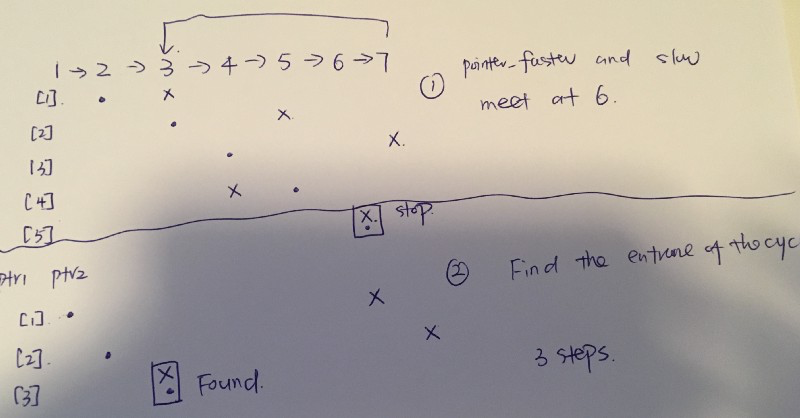
\includegraphics[width = 0.98\columnwidth]{fig/floyd.png}
    \caption{Example of floyd’s cycle finding}
    \label{fig:floyd}
\end{figure}

\begin{lstlisting}[language = Python]
def detectCycle(self, A):
        #find the "intersection" 
        p_f=p_s=A
        while (p_f and p_s and p_f.next):
            p_f = p_f.next.next
            p_s = p_s.next
            if p_f==p_s:
                break
        #Find the "entrance" to the cycle.
        ptr1 = A
        ptr2 = p_s;
        while ptr1 and ptr2:
            if ptr1!=ptr2:
                ptr1 = ptr1.next
                ptr2 = ptr2.next
            else:
                return ptr1
        return None
\end{lstlisting}
%%%%%%%%%%%%%%%%%%%%%%%%%%%%%%%%%%%%%%%%%%%%%%%%%%%%%%%%%%%%%%%%%%%%%%%%%%%%%%%%
% exercise
%%%%%%%%%%%%%%%%%%%%%%%%%%%%%%%%%%%%%%%%%%%%%%%%%%%%%%%%%%%%%%%%%%%%%%%%%%%%%%%%%%%
\section{Exercise}
\subsection{Number}
313. Super Ugly Number
\begin{lstlisting}
Super ugly numbers are positive numbers whose all prime factors are in the given prime list primes of size k. For example, [1, 2, 4, 7, 8, 13, 14, 16, 19, 26, 28, 32] is the sequence of the first 12 super ugly numbers given primes = [2, 7, 13, 19] of size 4.

Note:
 (1) 1 is a super ugly number for any given primes.
 (2) The given numbers in primes are in ascending order.
 (3) 0 < k <= 100, 0 < n <= 106, 0 < primes[i] < 1000.
 (4) The nth super ugly number is guaranteed to fit in a 32-bit signed integer.
\end{lstlisting}
\begin{lstlisting}[language=Python]
def nthSuperUglyNumber(self, n, primes):
        """
        :type n: int
        :type primes: List[int]
        :rtype: int
        """
        nums=[1]
        idexs=[0]*len(primes) #first is the current idex
        for i in range(n-1):
            min_v = maxsize
            min_j = []
            for j, idex in enumerate(idexs):
                v = nums[idex]*primes[j]
                if v<min_v:
                    min_v = v
                    min_j=[j]
                elif v==min_v:
                    min_j.append(j) #we can get mutiple j if there is a tie
            nums.append(min_v)
            for j in min_j:
                idexs[j]+=1 
        return nums[-1]
\end{lstlisting}
\end{document}